\subsection{Architecture}

\begin{figure}[h]
    \centering
    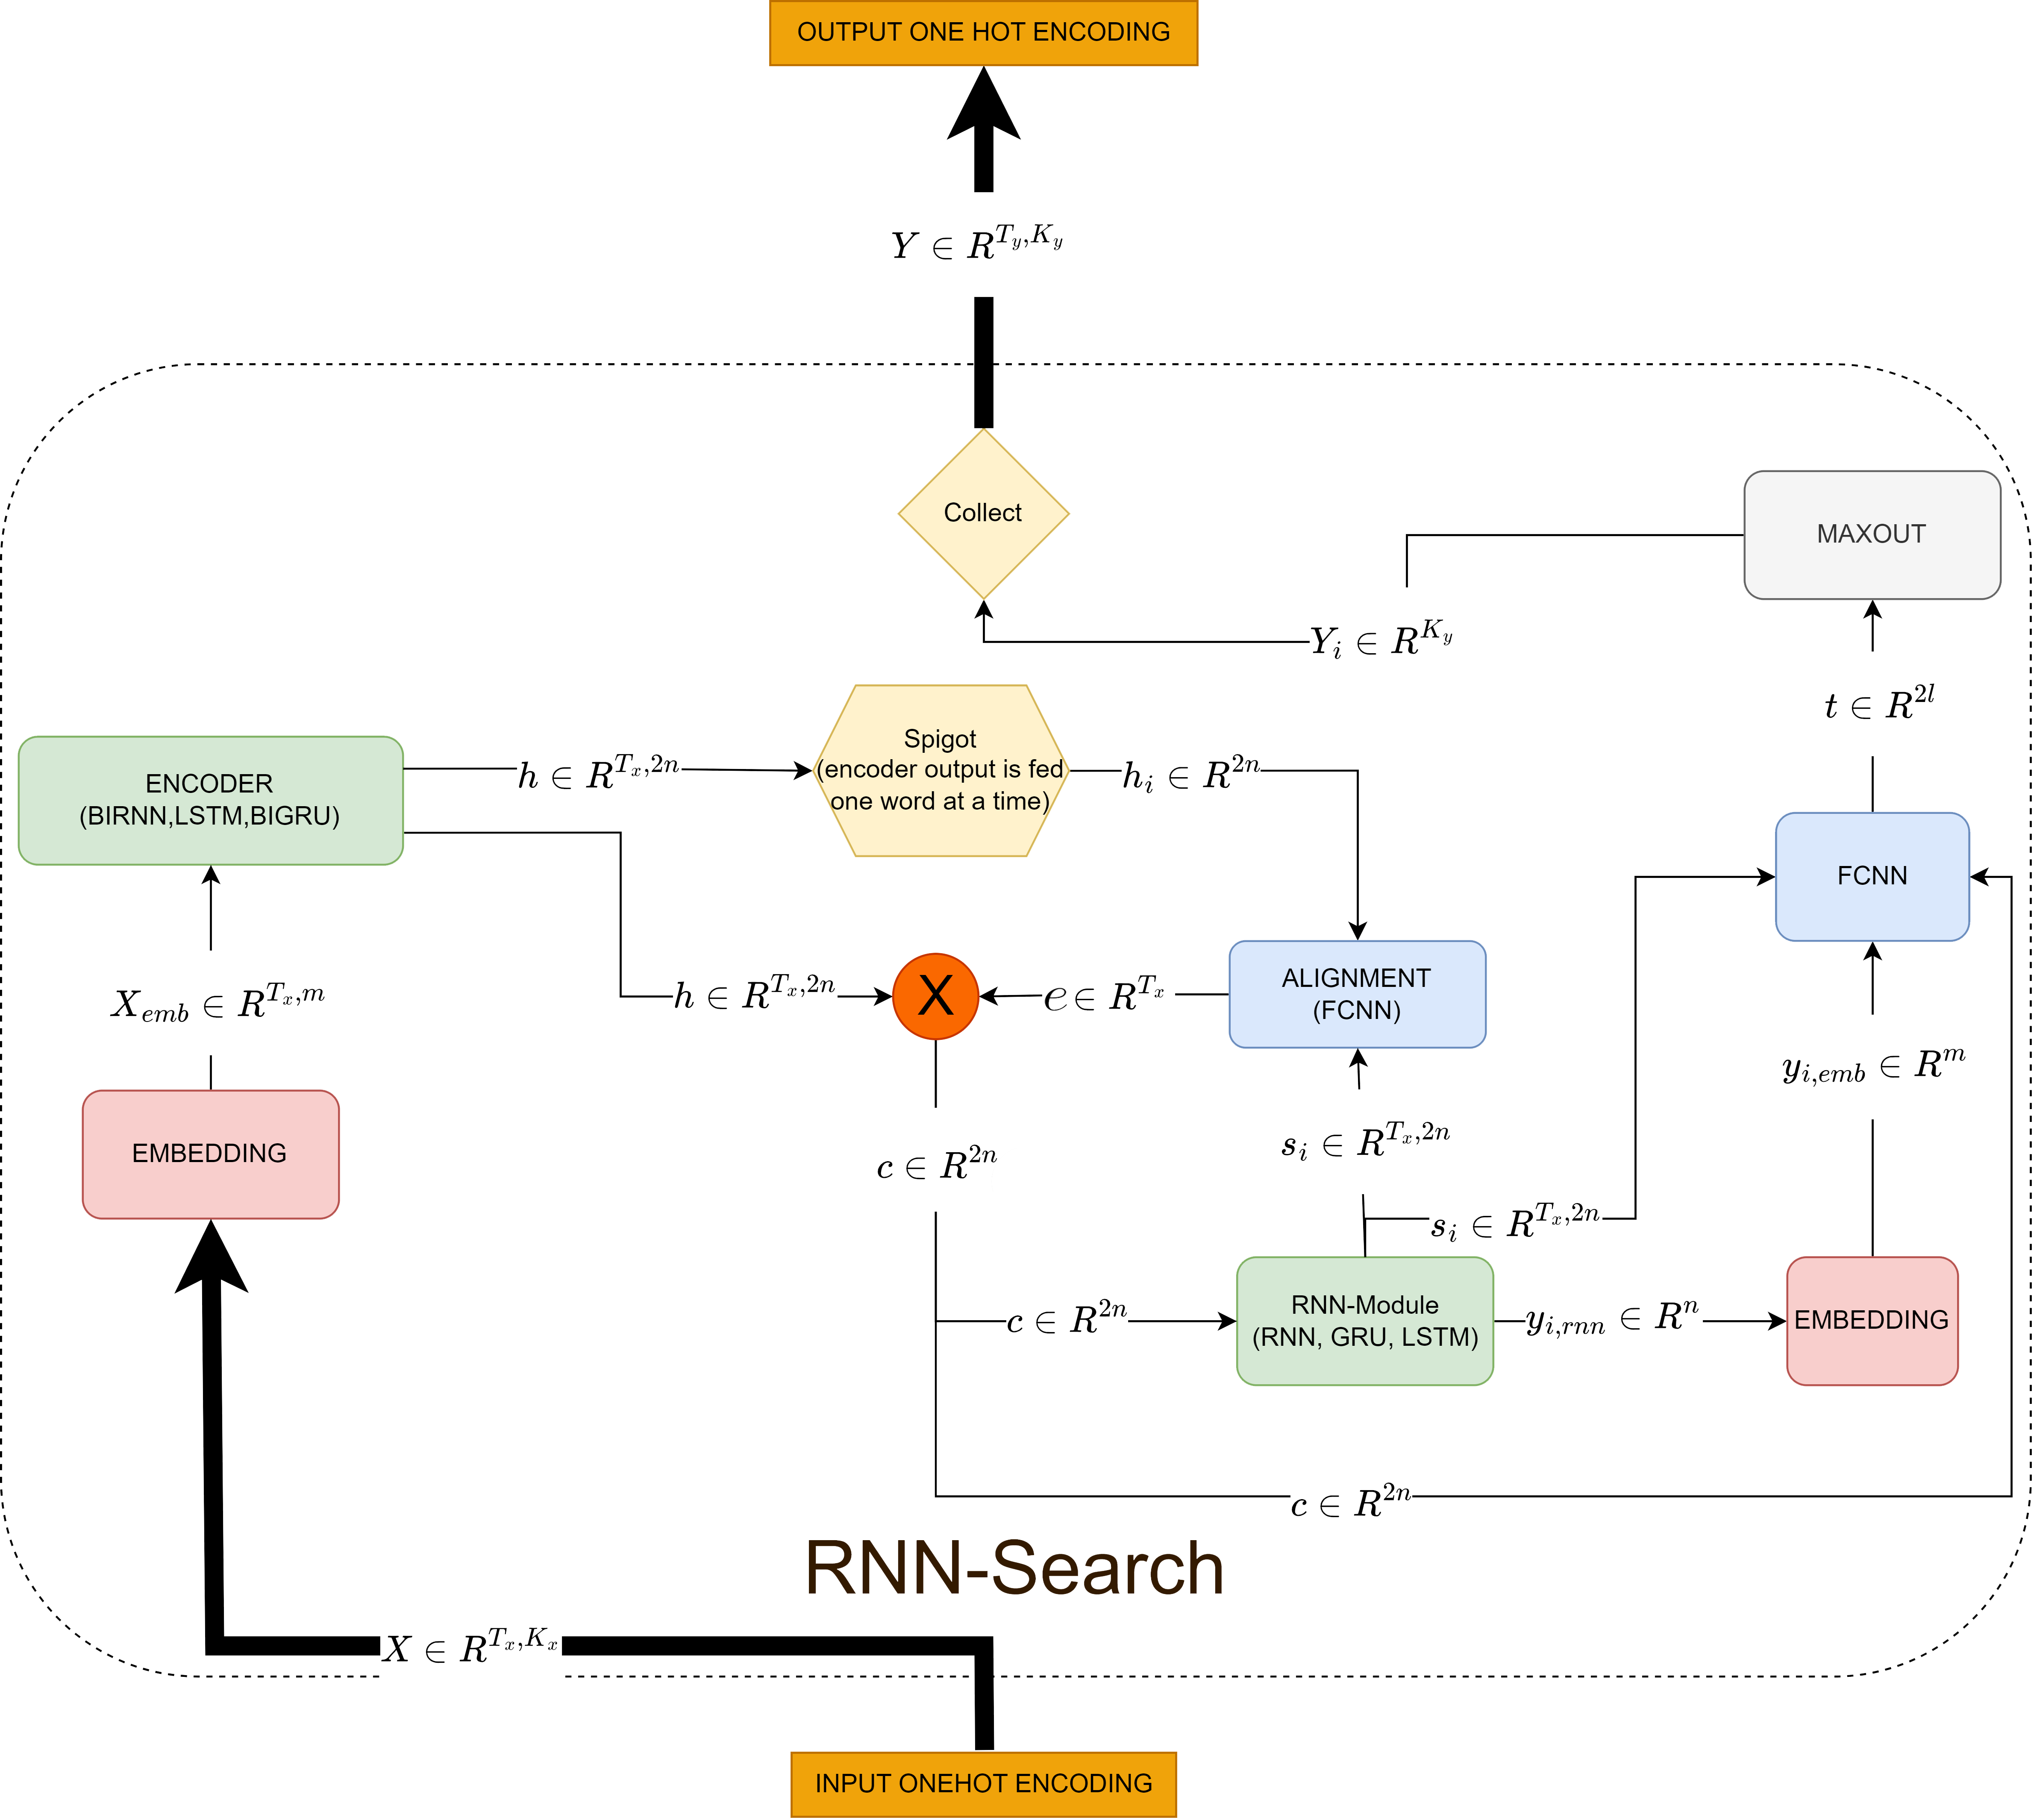
\includegraphics[width=\textwidth]{architecture.png}
    \caption{General Presentation of the Used architecture}
    \label{fig:architecture}
\end{figure}

In my approach, I tried to be as close as possible to the article's proposed architecture \ref{fig:architecture}. The model was organized into two main modules: An encoder and a decoder. On one hand, the encoder takes one-hot encoding representation of the input English phrase, reduces its dimension, then applies an RNN type module. On the other hand, the decoder takes the sequence of vectors given by the encoder, and one vector at a time calculates some weights to be used to modify the input vectors into one context vector that is used to predict the current word after being passed through a maxout layer.



\subsection{Approach Overview}

The paper introduces an innovative approach to enhance existing machine translation models, diverging from both statistical models and Encoder-Decoder architectures. The approach can be divided into the following substeps:

\subsubsection{Phrase Encoding}

The initial step involves encoding the input phrase using a Bag-of-Words representation. The vocabulary for this representation is derived either from the web, encompassing the most common 30,000 English/French words, or by utilizing the training set alone, or in combination with the test set. Each word in a phrase is then represented by indices in the vocabulary. Words without corresponding entries in the current vocabulary are mapped to the \textbf{\textless UNK\textgreater} token. Sentence padding is applied without an \textbf{\textless EOS\textgreater} token index, with the expectation that the model learns when to conclude. Consequently, each phrase is represented by a tensor of size $R^{T_x}$.

\subsubsection{Embedding and Encoding}

For efficient preprocessing, multiprocessing (except on Linux due to incompatibility) and HuggingFace's \textbf{.map} method are employed, significantly expediting data processing. The representation undergoes transformation through an embedding layer, resulting in a vector of size $R^{T_x,m}$. This vector is directly fed into the Bi-RNN unit of the encoder, producing an output of size $R^{T_x,2n}$ and an unused hidden state.

\subsubsection{Decoding and Maxout}

In a sequential manner, the encoder's output vectors $h_i$ are fed into the decoder module. Initially, the Alignment network generates weights of size $R^{T_x}$. These weights combine the $h$ vectors into a context vector $c$, which is then supplied to the RNN section of the decoder. Post-decoding, the hidden state of the RNN, its output $y_{i,rnn}$ (compressed to the size of the embedding $m$), and the context vector are processed through a single Fully Connected layer. Subsequently, the output undergoes a max-out layer, halving its dimension, followed by a "relaxation" layer to achieve the desired shape of $R^{K_y}$. This representation signifies the probability of $y_i$ representing each word in the vocabulary, with the omission of softmax until the application of the Negative Log Loss in the loss criterion. After predicting $y_i$ for $i \in [1:T_y]$, we backpropagate the loss along with L2 regularization loss taken with respect to all model parameters.

\subsection{Detailed Architecture}

We'll be using the following notations: $T_x, T_y$ sequence length of input and output respectively. $K_x, K_y$ vocabulary sizes used for input and output respectively. $m$ is the embedding size, $n$ is the hidden dimension size in both the encoder's RNN and that of the decoder, and $l$ is a latent dimension used in the MaxOut module.
\subsubsection{RNNSearch Translation Model}
\begin{enumerate}
    \item \textbf{Embedding layers ($E_1$ and $E_2$)}: used to reduce the dimension of the input one-hot encoded vector from $T_x$, can be represented by two 2D matrices or a single dense layer with no activation function and no bias.
    
    \item \textbf{Encoder's BiRNN layer (We use GRU as the RNN module)}: We do not directly use the hidden state of the encoder, only the output of size $R^{T_x,2n}$.
    
    \item \textbf{Alignment network}: The main contribution of the paper. Used to calculate the weights corresponding to each part of the sentence $\in R^{T_x}$. Uses the current hidden state of the decoder's RNN and the corresponding decoder's output.
    
    \item \textbf{Decoder's RNN}: used in a one-step-at-a-time fashion (feeding only sequences of length 1) to be able to modify the next input with a context vector generated from the alignment network.
    
    \item \textbf{Maxout Unit}: combines outputs from the decoder's RNN, the predicted word, and the context vector. It implements the maxout activation with two units as described in \cite{Goodfellow-et-al-2016}.
\end{enumerate}
\subsubsection{RNNEncoDeco Translation Model}
We by pass all connections used previously in RNNSearch and directly apply the RNN layer of the decoder to the encoder's output then apply a "relaxation" layer and a softmax to get the probabilities of predicting a word in the vocabulary.

\subsection{Training}

\begin{enumerate}
    \item \textbf{Cost Function:} We experiment with both : Negative log-likelihood and Cross Entropy Loss. To that we add an L2 regularization over all the parameters of the model with a weight of $10^{-4}$
    
    \item \textbf{Optimization}: Since Adadetla used in the article is a special case of Adam without the first order smoothing, we expirement with both.
    
    \item \textbf{Checkpointing:} we save a copy of our model everytime the loss on the validation gets smaler after an entire epoch

    \item \textbf{Framework:} We completely rely on pytorch for it's compatibality and ease of use. 
    
    \item  \textbf{Unitary Testing:} For each of the implemented modules we implement a corresponding unit test that insures types, intialization and tensor shapes. 
    
\end{enumerate}

\subsection{Inference (Translation)}

when it comes to predicting phrases, we rely on an optimized version of beam search that implements rejection of consecutive parts repition within a sentence with beam length of 5.
We also tried with argmax to predict indicies but results weren't always coherent

